\section{Preliminaries}\label{sec:model}
Our algorithm computes the value functions that dynamic programming
passes between parts of a sparse problem. We first state the problem and
show why it is easy once the support is fixed. We then run dynamic
programming by hand on a chain of variables, where the basic difficulty
already appears: the eliminated part must be summarized by a function of
a continuous variable, and its optimal support changes with that
variable. Tree decompositions extend this to general sparse matrices,
where the number of such supports can become exponential.
Sections~\ref{sec:prelim-messages} and~\ref{sec:main-result} define the
messages we compute, describe the perturbation, and outline the proof of
the main result.

\subsection{The problem}\label{sec:prelim-problem}
For $n\ge1$, the \emph{indicator quadratic problem} is
\begin{equation}\label{eq:problem}
 v_\xi=\min\left\{x^TQx+c^Tx+(\lambda+\xi)^Tz:
 x\in\R^n,\ z\in\{0,1\}^n,\ x_i(1-z_i)=0\ (i\in[n])\right\}.
\end{equation}
Here $[n]=\{1,\ldots,n\}$, $Q\in\Q^{n\times n}$ is symmetric, and
$c,\lambda\in\Q^n$. Each continuous variable $x_i$ has a binary indicator
$z_i$. The constraint $x_i(1-z_i)=0$ allows $x_i\ne0$ only if $z_i=1$,
and the choice $z_i=1$ costs the penalty $\lambda_i+\xi_i$. The penalties
$\lambda_i$ may have either sign. The vector $\xi\in\Q^n$ is the
\emph{perturbation} of the penalties, and $\xi=0$ gives the original
problem. Section~\ref{sec:main-result} describes how $\xi$ is drawn at
random, and the exact results of Section~\ref{sec:spectral} concern the
perturbed problem. We are given rational bounds
\begin{equation}\label{eq:spectral}
 0<\mu I\preceq Q\preceq HI,\qquad |c_i|\le C\quad(i\in[n]).
\end{equation}
Thus $Q$ is positive definite with all eigenvalues in $[\mu,H]$. These
numbers enter the running-time bound of Theorem~\ref{thm:main}. All norms
are Euclidean unless stated otherwise. For index sets $A,B\subseteq[n]$,
we write $Q_{AB}$ for the submatrix of $Q$ with rows in $A$ and columns
in $B$, and $x_A$ for the subvector of $x$ indexed by $A$.

The \emph{support} of a feasible pair $(x,z)$ is $A=\{i:z_i=1\}$, and a
coordinate $i$ is \emph{active} if $z_i=1$. The constraint
$x_i(1-z_i)=0$ forces $x_i=0$ only for inactive coordinates. An active
coordinate may therefore be zero, and the support need not equal
$\{i:x_i\ne0\}$. For instance, if $\lambda_i+\xi_i<0$, activating $i$
lowers the cost even if $x_i$ stays zero.

Once the support is fixed, the problem is easy. For a support $A$, the
inactive coordinates are zero, and what remains is the minimization of
$x_A^TQ_{AA}x_A+c_A^Tx_A$ over $x_A\in\R^A$. The matrix $Q_{AA}$ is a
principal submatrix of $Q$, hence positive definite, so this quadratic is
strictly convex. Setting its gradient $2Q_{AA}x_A+c_A$ to zero gives a
linear system, whose solution and optimal value are
\[
 x_A=-\tfrac12Q_{AA}^{-1}c_A,\qquad
 x_A^TQ_{AA}x_A+c_A^Tx_A=-\tfrac14c_A^TQ_{AA}^{-1}c_A.
\]
The optimum $v_\xi$ is therefore the least of the $2^n$ numbers
$-\frac14c_A^TQ_{AA}^{-1}c_A+\sum_{i\in A}(\lambda_i+\xi_i)$, one for each
support $A\subseteq[n]$, where the empty support has value zero. All the
difficulty lies in choosing the support.

When $Q$ is sparse, this choice can be made one group of variables at a
time. The sparsity pattern is described by the \emph{support graph} of
$Q$, which has vertex set $[n]$ and an edge $ij$ for each pair $i\ne j$
with $Q_{ij}\ne0$. Two variables are adjacent exactly when the objective
contains their product.

\subsection{Dynamic programming on a chain}\label{sec:prelim-chain}
Suppose first that $Q$ is tridiagonal, that is, $Q_{ij}=0$ whenever
$|i-j|>1$, so that the support graph is contained in the path
$1,2,\ldots,n$. Such matrices arise, for example, when $x_i$ is the value
of a signal at time $i$ and the objective couples consecutive times.
Write $\rho_i=\lambda_i+\xi_i$. The objective of \eqref{eq:problem} is then
\begin{equation}\label{eq:chain-objective}
 \sum_{i=1}^n\bigl(Q_{ii}x_i^2+c_ix_i+\rho_iz_i\bigr)
 +\sum_{i=1}^{n-1}2Q_{i,i+1}x_ix_{i+1},
\end{equation}
so each pair $(x_i,z_i)$ interacts only with its neighbors in the chain.

Eliminate $(x_1,z_1)$ first. The terms that contain $x_1$ or $z_1$ are
$Q_{11}x_1^2+c_1x_1+\rho_1z_1+2Q_{12}x_1x_2$, and they involve the other
variables only through $x_2$. Fix $x_2=t$ and minimize over both choices
of $z_1$. If $z_1=0$, then $x_1=0$ and these terms vanish. If $z_1=1$,
they form a strictly convex quadratic in $x_1$, which is minimized at
$x_1=-(c_1+2Q_{12}t)/(2Q_{11})$. The least cost of the eliminated pair,
as a function of $t$, is therefore
\begin{equation}\label{eq:chain-first}
 M_1(t)=\min\left\{0,\ \rho_1-\frac{(c_1+2Q_{12}t)^2}{4Q_{11}}\right\}.
\end{equation}
The constant $0$ belongs to the empty support and the second quadratic to
the support $\{1\}$. Which of the two is smaller depends on $t$. Suppose
that $\rho_1>0$ and $Q_{12}\ne0$. The empty support is optimal where
$|c_1+2Q_{12}t|\le2\sqrt{Q_{11}\rho_1}$, and $\{1\}$ is optimal where the
reverse inequality holds. Both are optimal at the two points where
equality holds, which are irrational in general. Thus, already in this
smallest case, the optimal support changes with $t$ on every interval
$[-R,R]$ with $R$ large enough.

This is the essential difference from a discrete dynamic program. In a
shortest-path or knapsack recursion, the state passed from one stage to
the next takes finitely many values, and the recursion stores one number
per state. Here the state is the value $t$ of the continuous variable
$x_2$, which is decided only later, when the remaining variables are
optimized. The recursion must therefore keep the whole function $M_1$;
neither one number nor one best support describes the eliminated part.

Next eliminate $(x_2,z_2)$ with $x_3=t$ fixed. The cost of $(x_1,z_1)$ is
now summarized by $M_1(x_2)$, and the other terms that involve $x_2$ or
$z_2$ are $Q_{22}x_2^2+c_2x_2+\rho_2z_2+2Q_{23}x_2t$. Hence
\[
 M_2(t)=\min_{\substack{x_2\in\R,\ z_2\in\{0,1\}\\ x_2(1-z_2)=0}}
 \bigl\{M_1(x_2)+Q_{22}x_2^2+c_2x_2+\rho_2z_2+2Q_{23}x_2t\bigr\}.
\]
Choosing one of the two terms of the minimum \eqref{eq:chain-first} and a
value of $z_2$ fixes a support $A\subseteq\{1,2\}$. Once $A$ is fixed,
what remains is the minimization of a strictly convex quadratic in the
active variables among $x_1,x_2$, whose linear term depends affinely on
$t$, so its value is a quadratic function of $t$. Hence $M_2$ is the
minimum of four quadratics in $t$, one for each support of $\{1,2\}$.

Continuing in this way, suppose that $(x_1,z_1),\ldots,(x_k,z_k)$ have
been eliminated, where $k<n$. Their least cost depends on the remaining
variables only through $t=x_{k+1}$, and
\begin{equation}\label{eq:chain-k}
 M_k(t)=\min_{A\subseteq\{1,\ldots,k\}}F_A(t),
\end{equation}
where $F_A(t)$ is the least total of the terms that contain an
eliminated variable, given that the eliminated variables have support $A$
and $x_{k+1}=t$. By the closed form of
Section~\ref{sec:prelim-problem}, with $c_A$ replaced by
$c_A+2Q_{A,\{k+1\}}t$, each $F_A$ is a quadratic function of $t$; it is
given in general by \eqref{eq:noisybranch} below. Thus $M_k$ is the
minimum of up to $2^k$ quadratics, one for each support of the eliminated
variables, and each step computes $M_k$ from $M_{k-1}$ in the same way as
$M_2$ from $M_1$. After $n-1$ steps only $(x_n,z_n)$ remains, and
minimizing $M_{n-1}(x_n)+Q_{nn}x_n^2+c_nx_n+\rho_nz_n$ over it gives
$v_\xi$. If a support $A$ attains $M_{n-1}$ at an optimal choice of
$x_n$, then the minimizer with support $A$ gives optimal values of
$x_1,\ldots,x_{n-1}$.

Storing all $2^k$ quadratics is out of the question for large $k$, and on
a chain it is also unnecessary. Liu et al.\ solve the chain in quadratic
time as a shortest-path problem whose arcs are blocks of consecutive
active coordinates \cite{LiuPath}. This works because an inactive
coordinate is zero and splits the chain into independent blocks, so no
continuous value has to be passed across it. Bhathena et al.\ show that
on a chain, and more generally when the support graph of $Q$ is a tree,
these functions of one variable split into linearly many intervals,
each with a single quadratic piece; on a chain, each elimination step
adds at most two pieces
\cite[Proposition~1 and Lemmas~3 and~4]{BhathenaTrees}. Their algorithm
stores only these pieces, never forms the $2^k$ quadratics, and solves
the problem on trees in quadratic time \cite{BhathenaTrees}.

As noted in the Introduction, $M_k$ can be stored and reused when the
rest of the problem changes. If a variable $x_{n+1}$ is appended to the
chain, for example, only one more elimination step is needed, starting
from the stored $M_{n-1}$.

\subsection{Tree decompositions and separators}\label{sec:prelim-treedec}
On a chain, every block of eliminated variables touches the rest of the
problem through a single variable. For a general sparse matrix,
eliminating a set of variables leaves a function of all remaining
variables adjacent to that set, and the order of elimination decides how
many there are. Tree decompositions organize the elimination so that
this number stays small.

A \emph{tree decomposition} of the support graph is a tree whose nodes
$u$ carry vertex sets $B_u\subseteq[n]$, called \emph{bags}, such that
every vertex lies in some bag, both endpoints of every edge lie in a
common bag, and for each vertex the nodes whose bags contain it form a
connected subtree. We call the last condition the
\emph{running-intersection property}. The \emph{width} of the
decomposition is $\max_u|B_u|-1$, and the \emph{treewidth} of the graph
is the least width of a tree decomposition. A tree with at least one edge
has treewidth one, with one bag for each edge, so treewidth measures how
far a graph is from a tree.

We assume that a decomposition of width $w$ with $b$ bags is supplied.
For fixed $w$, such a decomposition can be computed in linear time when
one exists \cite{Bodlaender}. For example, if $Q$ has bandwidth $\beta$,
that is, $Q_{ij}=0$ whenever $|i-j|>\beta$, then the bags
$\{i,\ldots,\min\{i+\beta,n\}\}$ for $i=1,\ldots,n$, placed along a path,
form a tree decomposition of width at most $\beta$. A tree decomposition
whose tree is a path is a \emph{path decomposition}, and the least width
of a path decomposition is the \emph{pathwidth}. The chain of
Section~\ref{sec:prelim-chain} is the case $\beta=1$.
Figure~\ref{fig:treedec} shows the case $\beta=2$ and $n=6$, with the
bags $\{5,6\}$ and $\{6\}$ dropped because they lie inside $\{4,5,6\}$.
Tree decompositions are a standard tool for exploiting sparsity in
optimization. For example, Bienstock and Mu\~noz use them to build
polynomial-size linear programs that approximate mixed-integer polynomial
optimization problems whose constraint intersection graph has bounded
treewidth \cite{BienstockMunoz}.

\begin{figure}[t]
\centering
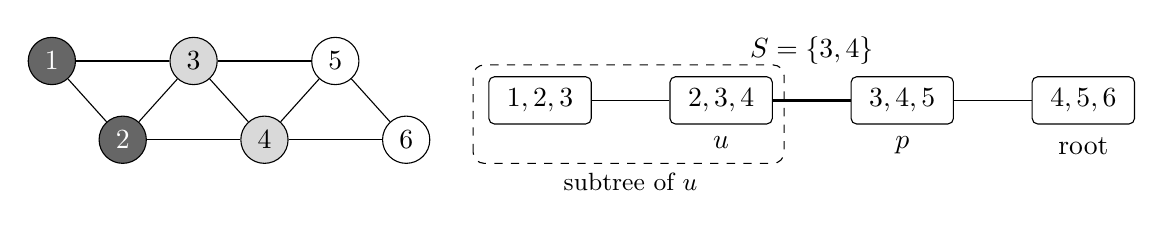
\begin{tikzpicture}[
 vtx/.style={circle,draw,minimum size=6mm,inner sep=0pt},
 int/.style={vtx,fill=black!60,text=white},
 sep/.style={vtx,fill=black!15},
 bag/.style={draw,rounded corners=2pt,minimum height=6mm,
             minimum width=13mm,inner sep=2pt}]
 \node[int] (v1) at (0,1) {$1$};
 \node[int] (v2) at (0.9,0) {$2$};
 \node[sep] (v3) at (1.8,1) {$3$};
 \node[sep] (v4) at (2.7,0) {$4$};
 \node[vtx] (v5) at (3.6,1) {$5$};
 \node[vtx] (v6) at (4.5,0) {$6$};
 \foreach \a/\b in {v1/v2,v2/v3,v3/v4,v4/v5,v5/v6,v1/v3,v2/v4,v3/v5,v4/v6}
  \draw (\a) -- (\b);
 \begin{scope}[shift={(6.2,0.5)}]
  \node[bag] (b1) at (0,0) {$1,2,3$};
  \node[bag] (b2) at (2.3,0) {$2,3,4$};
  \node[bag] (b3) at (4.6,0) {$3,4,5$};
  \node[bag] (b4) at (6.9,0) {$4,5,6$};
  \draw (b1) -- (b2);
  \draw[line width=1.2pt] (b2) -- node[above=9pt] {$S=\{3,4\}$} (b3);
  \draw (b3) -- (b4);
  \node[below=1pt] at (b2.south) {$u$};
  \node[below=1pt] at (b3.south) {$p$};
  \node[below=1pt] at (b4.south) {root};
  \draw[dashed,rounded corners=4pt] (-0.85,-0.8) rectangle (3.1,0.45);
  \node[anchor=north] at (1.15,-0.8) {\small subtree of $u$};
 \end{scope}
\end{tikzpicture}
\caption{Left: the support graph of a $6\times6$ matrix of bandwidth two.
Right: a tree decomposition of width two whose bags $\{i,i+1,i+2\}$,
$i=1,\ldots,4$, are the triangles of the graph, placed along a path and
rooted at $\{4,5,6\}$. For the node $u$ with parent $p$, the separator is
$S=B_u\cap B_p=\{3,4\}$ (light) and the internal set is $I=\{1,2\}$
(dark). The variables $x_1,x_2$ interact with $x_5,x_6$ only through
$x_3,x_4$.}
\label{fig:treedec}
\end{figure}

The edges of a rooted decomposition give the separators. Root the
supplied decomposition at any node. For a non-root node $u$ with parent
$p$, let $S=B_u\cap B_p$, and let $I$ be the set of vertices that lie in
a bag of the subtree rooted at $u$ but not in $S$. We call $S$ the
\emph{separator} and $I$ the \emph{internal set} of $u$. No edge of the
support graph joins $I$ to $[n]\setminus(I\cup S)$, so the variables in
$I$ interact with the rest of the problem only through those in $S$.
Indeed, suppose $ij$ is such an edge with $i\in I$, and take a bag
containing both endpoints. If the bag lies in the subtree of $u$, then
$j\in I\cup S$. Otherwise $i$ lies in bags on both sides of the tree edge
$up$, so the running-intersection property gives $i\in B_u\cap B_p=S$.
Both cases contradict the choice of $ij$. For the chain, with the bags
$\{i,\min\{i+1,n\}\}$ rooted at the last bag $\{n\}$, the node with bag
$\{k,k+1\}$ has separator $\{k+1\}$ and internal set $\{1,\ldots,k\}$,
which is exactly the situation after $k$ elimination steps.

\subsection{Messages, branches, and dictionaries}
\label{sec:prelim-messages}
The value functions $M_k$ of the chain generalize as follows. Let
$I,S\subseteq[n]$ be disjoint; the main case is the internal set and the
separator of a node of the decomposition
(Section~\ref{sec:prelim-treedec}). Write $t$ for the boundary values
$x_S$, and fix a box radius $R\ge0$. The \emph{message} is the
conditional value function
\begin{equation}\label{eq:message}
 M_{I,S}(t)=\min_{\substack{x_I\in\R^I,\ z_I\in\{0,1\}^I\\
                     x_i(1-z_i)=0\ (i\in I)}}
 \left\{x_I^TQ_{II}x_I+(c_I+2Q_{IS}t)^Tx_I
           +\sum_{i\in I}(\lambda_i+\xi_i)z_i\right\},
 \qquad t\in[-R,R]^{|S|}.
\end{equation}
The message keeps exactly the objective terms that involve an internal
variable: the internal quadratic, the coupling $2t^TQ_{SI}x_I$, and the
internal linear terms and penalties. It leaves out the boundary unary
terms $Q_{ss}t_s^2+c_st_s$ ($s\in S$), the edges within $S$, and the
boundary penalties. For fixed boundary variables $(x_S,z_S)$, these terms
add the same amount to every internal solution, so they do not change
which internal support is optimal. They are counted once, with the rest
of the problem. On the box, the function $M_k$ of the chain is the message
with $I=\{1,\ldots,k\}$ and $S=\{k+1\}$. The radius $R$ is part of the
input, and the running time of Section~\ref{sec:spectral} grows
polynomially with $R$ at fixed width. The radius $R=nC/(2\mu)$ suffices
for optimization: for every $\xi$, this box contains the boundary values
$x_S$ of every optimal solution (Section~\ref{sec:spectral-bounds}).

Now let $S$ and $I$ be the separator and internal set of a non-root node
$u$ of the rooted decomposition. Fix all variables outside $I$, with
$x_S=t\in[-R,R]^{|S|}$. Since no edge joins $I$ to a vertex outside
$I\cup S$, the objective of \eqref{eq:problem} equals the objective in
\eqref{eq:message} plus terms that do not involve $(x_I,z_I)$. Minimizing
over $(x_I,z_I)$ therefore gives $M_{I,S}(t)$ plus those terms. Thus
$M_{I,S}$ is the exact subtree message: it is all that the rest of the
problem needs to know about the subtree. We also include the root
message $M_{[n],\varnothing}$. Its box is a single point, and its value
is the global optimum $v_\xi$. In total there are at most $b$ messages,
each with $|S|\le w+1$.

Boundary indicators need no separate messages. The internal problem
depends on the boundary only through $t=x_S$. A boundary indicator $z_s$
only decides whether $t_s$ may be nonzero and adds the penalty
$\lambda_s+\xi_s$, which lies outside the message. For each assignment of
the boundary indicators, the contribution of the subtree is therefore
$M_{I,S}$ restricted to the slice of the box where $t_s=0$ whenever
$z_s=0$. One dictionary serves all $2^{|S|}$ assignments.

For a fixed support $A\subseteq I$, the coordinates of $I$ outside $A$
are zero, and the closed form of Section~\ref{sec:prelim-problem}, with
$c_A$ replaced by $c_A+2Q_{AS}t$, gives the minimizer and the value:
\begin{align}
 x_A(t)&=-\tfrac12Q_{AA}^{-1}(c_A+2Q_{AS}t),\label{eq:optimizer}\\
 q_A(t)&=-\tfrac14(c_A+2Q_{AS}t)^TQ_{AA}^{-1}
                    (c_A+2Q_{AS}t)+\sum_{i\in A}\lambda_i,\label{eq:branch}\\
 F_A(t)&=q_A(t)+\sum_{i\in A}\xi_i,\label{eq:noisybranch}\\
 M_{I,S}(t)&=\min_{A\subseteq I}F_A(t).
 \label{eq:envelope}
\end{align}
We call $q_A$ and $F_A$ the unperturbed and perturbed \emph{branches} of
$A$; they agree when $\xi=0$. The word refers to one term of the minimum
\eqref{eq:envelope}, not to branching in branch-and-bound. The empty
support has $q_\varnothing=F_\varnothing=0$. Each branch is a concave
quadratic in $t$, because $Q_{AA}^{-1}$ is positive definite. It is a
\emph{full} quadratic: one polynomial formula on all of $\R^{|S|}$, not
only on the region where $A$ is optimal. Its coefficients are rational
when $\xi$ is rational. In the first step of the chain,
\eqref{eq:chain-first} lists the two branches $F_\varnothing=0$ and
$F_{\{1\}}$ of the message with $I=\{1\}$ and $S=\{2\}$.

By \eqref{eq:envelope}, a message is the pointwise minimum of $2^{|I|}$
branches, but only some of them are needed. A \emph{dictionary} for
$M_{I,S}$ is a set of perturbed branches $F_A$, each stored with its
support $A$, whose pointwise minimum equals $M_{I,S}$ on
$[-R,R]^{|S|}$. A support $A$ is \emph{optimal somewhere} on the box if
$F_A(t)=M_{I,S}(t)$ for at least one $t$ in the box. Branches whose
supports are never optimal on the box can be dropped without changing
the message there.

A dictionary may still contain supports that are never optimal on the
box, and it does not describe the region where each branch is optimal.
These regions can end at irrational points, as already in
\eqref{eq:chain-first}. Everything a dictionary stores is rational.
Hence, at a rational $t$ in the box, the least branch value gives
$M_{I,S}(t)$ exactly, and \eqref{eq:optimizer} for a minimizing support
gives an optimal internal solution. The dictionaries of
Section~\ref{sec:spectral} contain every support optimal somewhere,
including supports optimal only at a single tie point, so at every
boundary value in the box they give all optimal internal supports, not
just one.

Exact dynamic programming computes the messages from the leaves of the
rooted decomposition toward the root, as on the chain. Let $u$ be a node
with separator $S$ and internal set $I$ (for the root, take
$S=\varnothing$ and $I=[n]$). Let $v_1,\ldots,v_r$ be its children, with
separators $S_j$ and internal sets $I_j$, and let $I_0=B_u\setminus S$
be the variables eliminated at $u$. Then $I$ is the disjoint union of
$I_0,I_1,\ldots,I_r$ by the running-intersection property: a vertex of
$B_u$ that lies in a bag in the subtree of $v_j$ also lies in $B_{v_j}$,
hence in $S_j=B_u\cap B_{v_j}$, so no $I_j$ meets $B_u$; a vertex in
bags in the subtrees of two different children lies in $B_u$, so it
lies in no $I_j$; and every vertex of $I$ outside $B_u$ lies in some
$I_j$. Each $S_j$ lies in $B_u=I_0\cup S$, so $x_{S_j}$ is determined by
$x_{I_0}$ and $t=x_S$. Splitting the terms of \eqref{eq:message}
accordingly gives
\[
 M_{I,S}(t)=\min_{\substack{x_{I_0}\in\R^{I_0},\
                     z_{I_0}\in\{0,1\}^{I_0}\\
                     x_i(1-z_i)=0\ (i\in I_0)}}
 \Bigl\{\Phi_u(x_{I_0},z_{I_0},t)
        +\sum_{j=1}^rM_{I_j,S_j}(x_{S_j})\Bigr\},
\]
where $\Phi_u(x_{I_0},z_{I_0},t)$ is the objective of \eqref{eq:message}
with $I$ replaced by $I_0$. Every term that involves a variable of
$I_j$, including its coupling with $x_{S_j}$, belongs to the child
message $M_{I_j,S_j}$. Each child message is given by the minimum in
\eqref{eq:message} at every $x_{S_j}\in\R^{|S_j|}$, not only on its box,
because $x_{S_j}$ may include coordinates of $x_{I_0}$, which range over
all of $\R$. The chain step from $M_{k-1}$ to $M_k$ is the case $r=1$
and $I_0=\{k\}$. Fixing a support $A_0\subseteq I_0$ and one branch
$F_{A_j}$ of each child fixes the internal support
$A=A_0\cup A_1\cup\cdots\cup A_r$. Minimizing
$\Phi_u+\sum_jF_{A_j}(x_{S_j})$ over $x_{I_0}$ with support $A_0$ then
gives $F_A(t)$, because each $F_{A_j}$ already minimizes over the
variables of $A_j$. Thus, if each child message is written, on all of
$\R^{|S_j|}$, as a minimum of $d_j$ branches, the message of $u$ is a
minimum of up to $2^{|I_0|}d_1\cdots d_r$ candidate branches. The exact
algorithm of Bhathena et al.\ forms these candidates and then discards
those that it identifies as never optimal on a box
\cite[Sections~4 and~5]{BhathenaStructured}.

The difficulty is the number of branches. A separator with $k$ variables
makes a message a function of $k$ variables, but it does not bound the
number of branches needed to represent it, even after pruning:
Section~\ref{sec:message-limits} gives, at width two, a message of one
boundary variable that needs exponentially many branches. The cause is
near ties among many supports. Bhathena et al.\ limit near ties by
conditions on the instance (Section~\ref{sec:related}); our main result
instead controls them by perturbing the penalties at random.

\subsection{The perturbation and an outline of the proof}
\label{sec:main-result}
Theorem~\ref{thm:main}, stated in Section~\ref{sec:spectral-main},
makes the main result of Section~\ref{sec:intro} precise. Each penalty
$\lambda_i$ is replaced by $\lambda_i+\xi_i$, where $\xi_1,\ldots,\xi_n$
are independent and uniform on the \emph{perturbation grid}
\begin{equation}\label{eq:noisegrid}
 \left\{-\sigma+\frac{2\sigma j}{N-1}:j=0,\ldots,N-1\right\}
\end{equation}
of $N$ equally spaced points in $[-\sigma,\sigma]$, including both
endpoints. Here $\sigma>0$ is rational and $N$ is the smallest power of
two with $N\ge2n$. Each $\xi_i$ therefore uses $\lceil\log_2(2n)\rceil$
random bits, and the perturbed penalties stay rational. The algorithm
uses $\xi$ only through $\lambda+\xi$, so it may draw $\xi$ itself or
receive an already perturbed instance. Running times are measured by bit
complexity, which counts bit operations and so accounts for the sizes of
all rational numbers that the algorithm forms.

The proof has four ingredients. The first is a counting argument at one
fixed boundary value $t$. The perturbation adds $\sum_{i\in A}\xi_i$ to
the cost of each support $A$. Fix all coordinates of $\xi$ except
$\xi_i$. If the best support that contains $i$ and the best one that
does not are both within $a$ of the optimum, then $\xi_i$ lies in a
fixed interval of length $2a$, which is unlikely when $a$ is small
compared with $\sigma$. Many near-optimal supports force this event for
many coordinates at once. Lemma~\ref{lem:count} makes this precise and
shows that the expected number of supports within $\sigma/(2n)$ of the
optimum at $t$ is at most $e\approx2.72$.

The second ingredient lists these supports. It needs only approximate
optimization, which matters because the solver we use for indicator
quadratics rounds the continuous variables to a finite grid. A
\emph{restricted additive oracle} is an algorithm that, with some
indicators fixed, returns a support consistent with them together with
its exact cost, which is within a given $\varepsilon$ of the best such
cost. Lawler's partition method splits the supports into cells by fixing
indicator bits, much like the subproblems of branch-and-bound, and
queries the oracle on each cell. Because each reported cost is exact and
within $\varepsilon$ of the best cost in its cell, the search can
certify when no near-optimal support remains. This certified version of
the method lists every support within $\sigma/(6n)$ of the optimum and
only supports within $\sigma/(2n)$ (Lemma~\ref{lem:enumeration}), so its
expected output size is at most $e$.

The third ingredient passes from one boundary value to the whole box. A
\emph{parameter net} is a finite set of points such that every point of
the box lies within a given distance of one of them. The branches are
Lipschitz on the box, so a support that is optimal at some $t$ is
near-optimal at a nearby net point. Running the enumeration at every
point of the net therefore finds every support optimal somewhere on the
box (Theorem~\ref{thm:dictionary}). Section~\ref{sec:enumeration} proves
these three ingredients for general families of supports, without
quadratics or graphs.

The fourth ingredient is the oracle itself. For indicator quadratics, a
dynamic program over a grid of continuous values on the tree
decomposition provides it (Lemma~\ref{lem:gridoracle}), and
Section~\ref{sec:spectral} combines it with the first three ingredients.
Each message is computed separately, without the exact recursion of
Section~\ref{sec:prelim-messages}: every oracle call for $M_{I,S}$
runs this grid dynamic program over all of $I$, so messages whose
subproblems overlap repeat work. The spectral bounds \eqref{eq:spectral}
control the Lipschitz constant of the branches and the grid resolution,
and the box must be bounded for the net to be finite. The width enters
as the exponent $w+1$ of the number of net points and of the size of
each grid table. The running-time bound of Theorem~\ref{thm:main} is
therefore polynomial for each fixed $w$, but its exponent depends on
$w$. It does not show fixed-parameter tractability in $w$, which would
require a bound $f(w)\,p$ with a polynomial $p$ whose degree does not
depend on $w$.
